\subsection{Torque Control}

The main attitude controller sends a torque demand to the actuators, which is then distributed between the actuators. Each of the reaction wheels get their own individual torque demand signals. Two methods have been implemented for tracking this torque demand. One is by transforming the torque to angular velocity demand, which the motor has to track, the other is directly controlling for actuator error.

\begin{figure}[h!]
	\centering 
	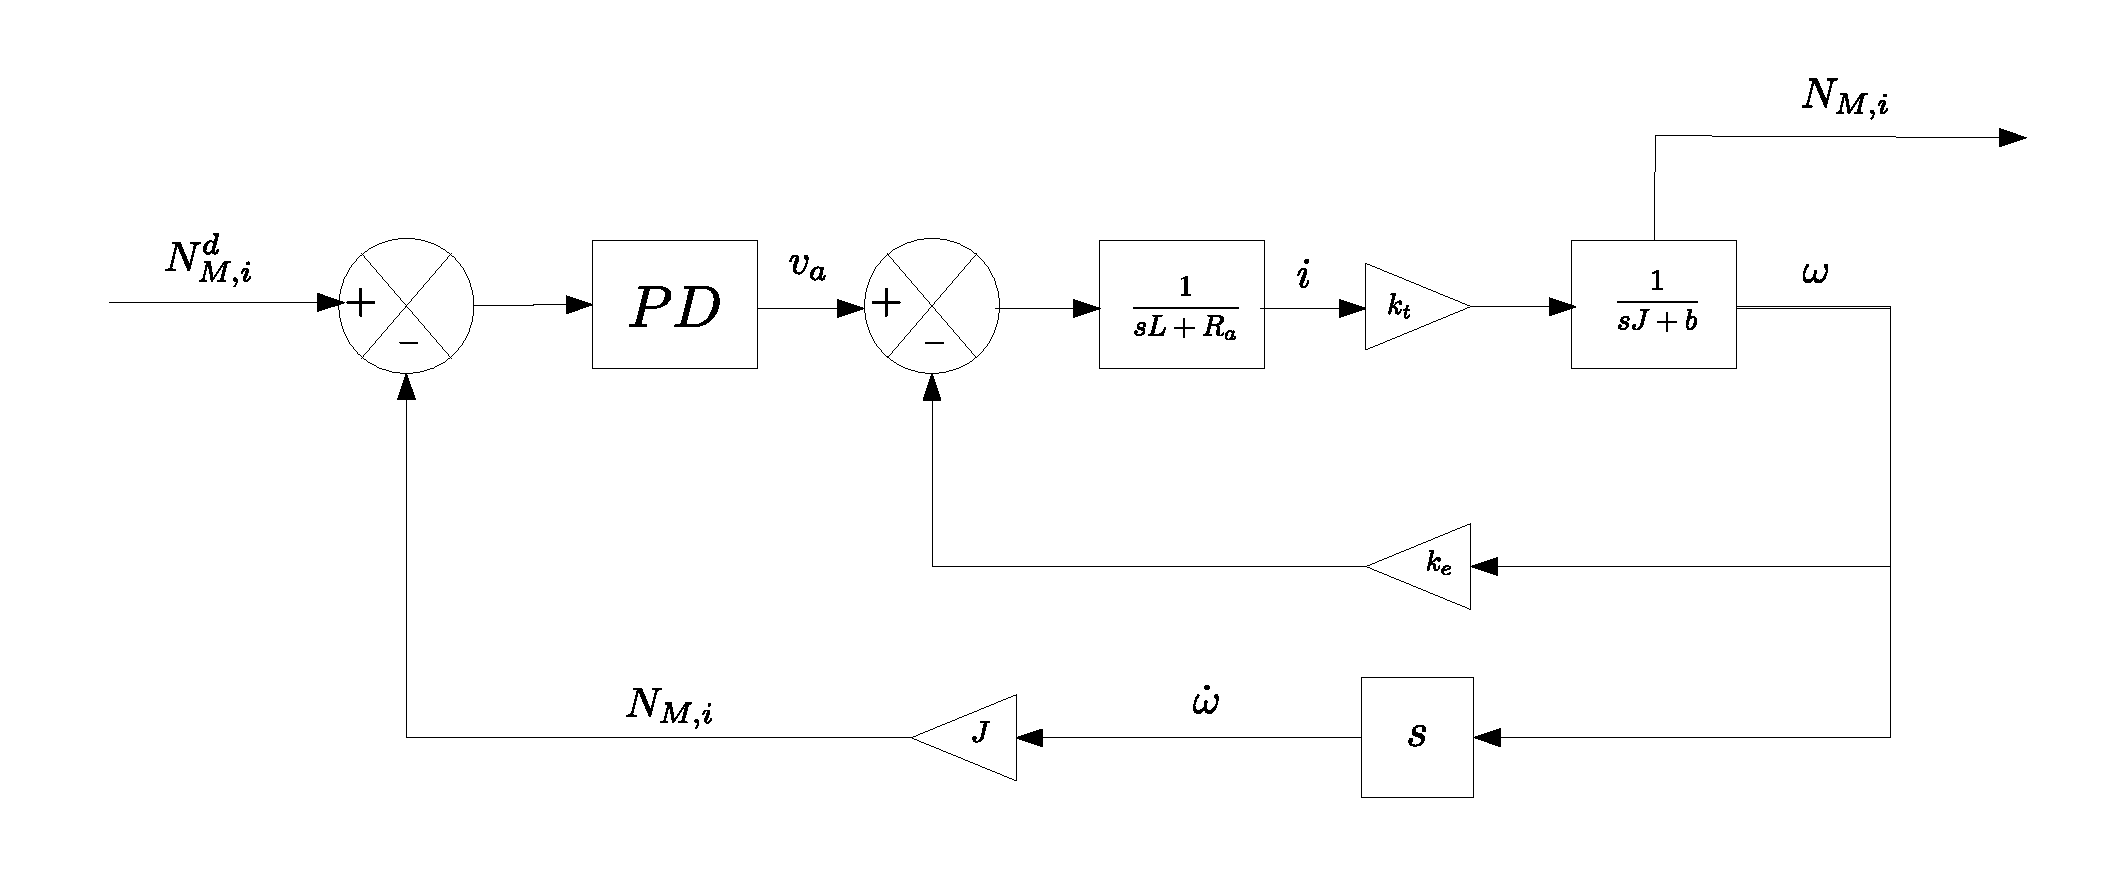
\includegraphics[width=170mm]{figures/torqueControl.pdf}	
	\caption{Torque control scheme.}
	\label{label{fig:torqueControl}}
\end{figure}

As shown on Figure \ref{fig:torqueControl} , the torque controller controls the torque error signal using a PD controller. Since the torque has a $ 10^{-5} Nm$ magnitude, while the voltage has $ 10^1 V$, numerically the PD gains are quite large. The control signal is the input voltage for the DC motor. The subsystem is second order, including an integrator for current and one for angular velocity.

\todo{PD calibration}